\section{Sensitivity analyses}
\label{sec:ablation}

The headline collapse (Claim~1) uses the cross-metal column, which is unaffected
by the choices below. We nonetheless bound the \emph{within-metal} column and the
corpus claim, because a reader is entitled to know where a conclusion is decided
by a preprocessing rule rather than by the data.

\subsection{The tie rule decides the Ru comparison}
\label{sec:ablation:tie}

When duplicate measurements of the same ligand disagree, the collapse rule
resolves an exact tie toward \emph{active} (predicate
$\text{sum}\times 2 \geq n$). This is the anti-conservative direction for an
activity claim, and it is the rule both the fingerprint probe and the neural
scorer use, so the within/cross comparison is internally consistent. But 80
ligands ($4.1\%$ of the deduplicated cohort) are exact ties, so it is worth
asking how much of the headline depends on the choice (Table~\ref{tab:tie}).

\begin{table}[t]
\centering
\caption{Within-metal AUC under the two tie rules. \MEASURED:
\texttt{metrics/by\_metric/metal\_activity\_transfer\_tie\_sensitivity.json}.}
\label{tab:tie}
\begin{tabular}{lcc}
\toprule
 & Ties $\to$ active (current) & Ties $\to$ inactive (conservative) \\
\midrule
Ru & $0.8128$--$0.8363$ & $0.7880$--$0.8082$ \\
Ir & $0.8295$--$0.8597$ & $0.8237$--$0.8374$ \\
\midrule
\multicolumn{3}{l}{Krasnov published: Ru $0.81$, Ir $0.73$} \\
\bottomrule
\end{tabular}
\end{table}

The consequence is asymmetric and we state it plainly. The \emph{Ir} claim is
robust: Ir exceeds $0.73$ under both rules and every seed. The \emph{Ru} claim is
\emph{not} robust: under the conservative rule Ru sits at $0.7880$--$0.8082$,
entirely at or just below $0.81$; under the current rule it sits at
$0.8128$--$0.8363$, entirely above. Whether Ru ``beats'' the published value is
decided by the tie rule, not by the chemistry. We therefore write Ru as
\emph{at parity} with $0.81$, and do not claim a win. The collapse itself is
unaffected, because it is a difference of two columns computed under the same
rule.

\subsection{Deduplication}
\label{sec:ablation:dedup}

Raw MetalCytoToxDB rows are heavily duplicated at the ligand level: Ru's
$3{,}668$ rows collapse to $1{,}255$ unique ligands ($65.8\%$ duplication), and
the duplication is uneven across metals. Both the within-metal and cross-metal
numbers are computed on the deduplicated cohort, so the two columns are
comparable to each other. Deduplication matters because the same ligand can be
measured against several metals; without it, a row split would put a ligand in
both train and test and inflate both columns. The LOMO protocol removes this
leak directly by dropping any training ligand that appears in the held-out
metal, so the cross-metal column is ligand-disjoint by construction.

\begin{figure}[t]
\centering
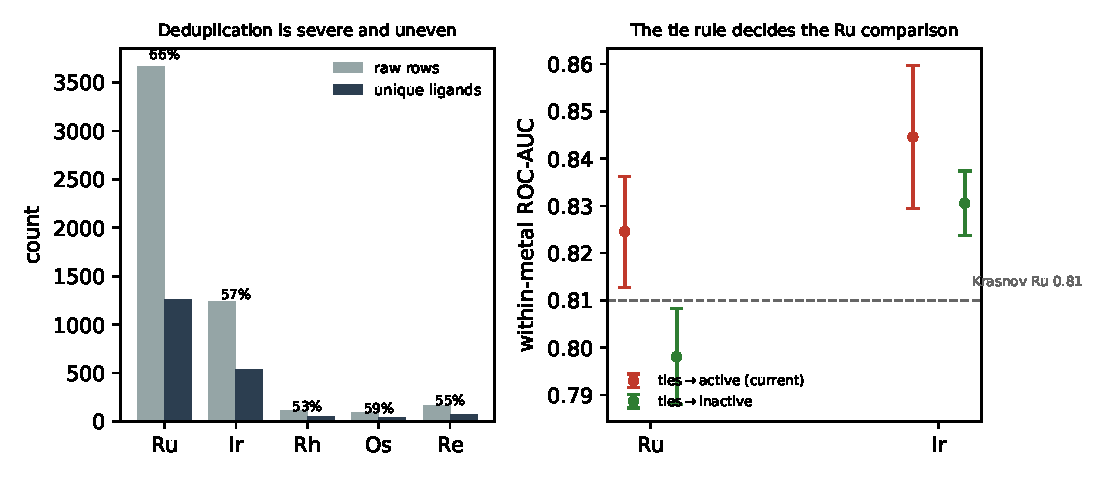
\includegraphics[width=0.95\linewidth]{fig3_dedup_tie.pdf}
\caption{Left: raw rows versus unique ligands per metal (percentage is the
duplication rate). Right: within-metal AUC interval across seeds under the two
tie rules; the Ru interval crosses the published $0.81$ line, the Ir interval
does not. \MEASURED:
\texttt{metrics/by\_metric/metal\_activity\_transfer\_seed\_stability.json},
\texttt{metal\_activity\_transfer\_tie\_sensitivity.json}.}
\label{fig:dedup}
\end{figure}

\subsection{Scorer choice}
\label{sec:ablation:scorer}

Claim~1's cross-metal column is measured with a Morgan-fingerprint plus XGBoost
probe. To show the collapse is not a fingerprint artefact we re-run the
ligand-disjoint LOMO evaluation with the official chemprop~v2 message-passing
backbone \citep{chemprop} on the same cohort and the same splits
(Table~\ref{tab:scorer}).

\begin{table}[t]
\centering
\caption{Scorer ablation on the Paper-A probe cohort: same cohort, same
ligand-disjoint LOMO split. Cross AUCs are 5-seed means for the backbone and a
single seed (42) for the fingerprint probe; the interval is a
$2{,}000$-resample bootstrap of the backbone's seed-42 cross ranking. The
verdict is a label-permutation null on that ranking, Holm--Bonferroni-corrected
over the five-metal family. \MEASURED:
\texttt{metrics/by\_metric/pa3\_chemprop\_lomo\_probe\_cohort.json}.}
\label{tab:scorer}
\begin{tabular}{lccccc}
\toprule
Metal & $n_{\text{test}}$ & Fingerprint & Backbone & Backbone 95\% CI & Holm $p$ \\
\midrule
Ru & $1{,}255$ & $0.6179$ & $0.5621$ & $[0.5075,0.5880]$ & $0.040$ \\
Ir & $534$      & $0.5276$ & $0.4841$ & $[0.4062,0.5033]$ & $0.228$ \\
Rh & $51$       & $0.5190$ & $0.4915$ & $[0.3243,0.6859]$ & $1.000$ \\
Os & $36$       & $0.4950$ & $0.5559$ & $[0.3311,0.7078]$ & $1.000$ \\
Re & $74$       & $0.4429$ & $0.7368$ & $[0.6202,0.8904]$ & $0.010$ \\
\bottomrule
\end{tabular}
\end{table}

The backbone reproduces the collapse on Ru, Ir and Rh (cross AUC $0.5621$,
$0.4841$, $0.4915$), keeps Os inside its null band, and recovers Re
($0.7368$). Under the family correction only Re and Ru survive: Ir's
below-chance reading under the backbone is significant only uncorrected
(one-sided $p=0.038$; two-sided $0.076$, Holm $0.23$). The collapse for Ru, Ir
and Rh is therefore robust to the scorer, while the Re exception is a property
of the representation, not of the metal axis. The within-metal column carries no
bootstrap interval here because the PA3 report stores per-fold AUCs but not the
per-ligand out-of-fold scores a within-metal bootstrap needs; the fingerprint
within column's interval is in \S\ref{sec:results:collapse}.

\subsection{tmQM bond-perception reference}
\label{sec:ablation:bond}

The tmQM corpus is the pretraining source for Claim~2 and, in a companion line
of work, the ground truth for metal bond-order perception. For completeness we
report the same-protocol bond-perception comparison on 900 held-out complexes
(150 per metal, non-hydrogen pair scope, per-complex aggregation,
Table~\ref{tab:bond}).

\begin{table}[t]
\centering
\caption{Bond perception on 900 held-out tmQM complexes, identical cohort and
per-complex aggregation for every column. The learned head and OpenBabel are
scored on non-hydrogen pairs; RDKit (stripped) is scored on its native
non-metal \emph{and} non-hydrogen pair scope. The head column is a mean $\pm$
sample std over three full-corpus checkpoints (seeds 0--2); OpenBabel and RDKit
are deterministic given the input, so their only uncertainty is the sampling of
the 900 complexes. \MEASURED:
\texttt{metrics/by\_metric/tmqm\_bond\_perception\_3seed.json}.}
\label{tab:bond}
\begin{tabular}{lccc}
\toprule
 & Learned head & OpenBabel \citep{openbabel} & RDKit (stripped) \citep{rdkit} \\
\midrule
bond EXISTENCE F1   & $\mathbf{0.9962 \pm 0.0008}$ & $0.9771$ & $0.9998$ \\
exact-type rate     & $\mathbf{0.0956 \pm 0.0113}$ & $0.0300$ & $0.0220$ \\
macro-F1(type)      & $0.4784 \pm 0.0055$ & $\mathbf{0.5051}$ & $0.2809$ \\
success rate        & $1.000$ & $1.000$ & $0.303$ \\
\bottomrule
\end{tabular}
\end{table}

The learned head wins two of three axes, including a $3.2\times$ edge in
exact-type rate, but it \emph{loses} the axis it was designed to win:
macro-F1(type) $0.4784 \pm 0.0055$ against OpenBabel's $0.5051$, $0.0267$ behind.
The loss is consistent across all three seeds and is nearly five times the
between-seed standard deviation, so it is not seed noise. We report the losing
row deliberately. We also record a withdrawn number: an earlier figure of
$0.9194$ came from a \emph{pooled} aggregation on a different cohort, and the
seed-0 checkpoint scores $0.4723$ under the per-complex protocol used here. The
two are not interchangeable, and quoting $0.9194$ beside OpenBabel's per-complex
$0.5051$ would compare three things at once.
